\newpage
\subsection{Caso d'uso UC2: Registrazione}
\begin{center}
	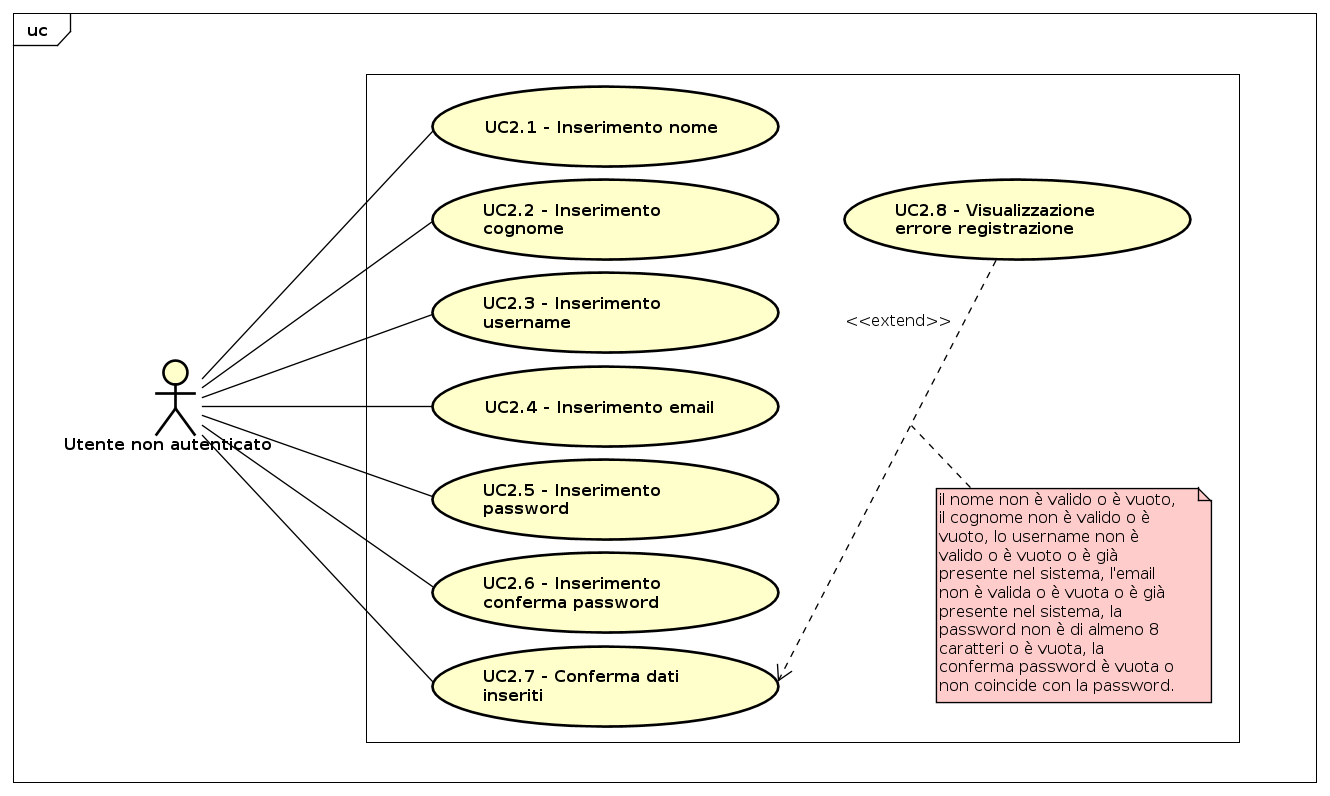
\includegraphics[scale=0.5]{UML/UC2.png}
\end{center}
\begin{itemize}
\item \textbf{Attori}: Utente;
\item \textbf{Scopo e descrizione}: per poter usufruire dei servizi forniti dalla piattaforma, l'utente deve registrarsi inserendo email e password;
\item \textbf{Precondizione}: il sistema è avviato e mostra la pagina iniziale;
\item \textbf{Scenario principale}:
	\begin{enumerate}
	\item L'utente inserisce il proprio nome (UCD2.1);
	\item L'utente inserisce il proprio cognome (UCD2.2);
	\item L'utente sceglie uno username (UCD2.3);
	\item L'utente inserisce l'email (UCD2.4);
	\item L'utente inserisce la password (UCD2.5);
	\item L'utente inserisce una seconda volta la password (UCD2.6);
	\item L'utente conferma i dati inseriti (UCD2.7).
	\end{enumerate}
\item \textbf{Scenario alternativo}: possono verificarsi uno o più dei seguenti scenari:
	\begin{itemize}
	\item[-] Il nome inserito non è valido oppure è vuoto;
	\item[-] Il cognome inserito non è valido oppure è vuoto;
	\item[-] Lo username inserito non è valido oppure è vuoto;
	\item[-] Lo username inserito è già presente nel sistema;
	\item[-] L'email inserita non è valida oppure è vuota;
	\item[-] L'email inserita è già presente nel sistema;
	\item[-] La password inserita è vuota oppure non è di almeno 8 caratteri;
	\item[-] La password e la conferma password non coincidono.
	\end{itemize}
In tal caso il sistema ritorna allo stato precedente l'inserimento dei dati visualizzando un messaggio di errore;
\item \textbf{Estensione}: l'utente visualizza un messaggio di errore (UCD2.8).
\item \textbf{Postcondizione}: il sistema ha registrato l'utente.
\end{itemize}

\subsubsection{Caso d'uso UC2.1: Inserimento nome}
\begin{itemize}
\item \textbf{Attori}: Utente;
\item \textbf{Scopo e descrizione}: l'utente inserisce il proprio nome per potersi registrare;
\item \textbf{Precondizione}: il sistema presenta all'utente lo spazio destinato a questa operazione;
\item \textbf{Postcondizione}: il nome è stato inserito.
\end{itemize}

\subsubsection{Caso d'uso UC2.2: Inserimento cognome}
\begin{itemize}
\item \textbf{Attori}: Utente;
\item \textbf{Scopo e descrizione}: l'utente inserisce il proprio cognome per potersi registrare;
\item \textbf{Precondizione}: il sistema presenta all'utente lo spazio destinato a questa operazione;
\item \textbf{Postcondizione}: il cognome è stato inserito.
\end{itemize}

\subsubsection{Caso d'uso UC2.3: Inserimento username}
\begin{itemize}
\item \textbf{Attori}: Utente;
\item \textbf{Scopo e descrizione}: l'utente inserisce il proprio username per potersi registrare;
\item \textbf{Precondizione}: il sistema presenta all'utente lo spazio destinato a questa operazione;
\item \textbf{Postcondizione}: lo username è stato inserito.
\end{itemize}

\subsubsection{Caso d'uso UC2.4: Inserimento email}
\begin{itemize}
\item \textbf{Attori}: Utente;
\item \textbf{Scopo e descrizione}: l'utente inserisce il proprio indirizzo email per potersi registrare;
\item \textbf{Precondizione}: il sistema presenta all'utente lo spazio destinato a questa operazione;
\item \textbf{Postcondizione}: l'email è stata inserita.
\end{itemize}

\subsubsection{Caso d'uso UC2.5: Inserimento password}
\begin{itemize}
\item \textbf{Attori}: Utente;
\item \textbf{Scopo e descrizione}: l'utente inserisce una password a sua scelta per potersi registrare;
\item \textbf{Precondizione}: il sistema presenta all'utente lo spazio destinato a questa operazione;
\item \textbf{Postcondizione}: la password è stata inserita.
\end{itemize}

\subsubsection{Caso d'uso UC2.6: Inserimento conferma password}
\begin{itemize}
\item \textbf{Attori}: Utente;
\item \textbf{Scopo e descrizione}: l'utente inserisce nuovamente la password scelta;
\item \textbf{Precondizione}: il sistema presenta all'utente lo spazio destinato a questa operazione;
\item \textbf{Postcondizione}: la conferma della password è stata inserita.
\end{itemize}

\subsubsection{Caso d'uso UC2.7: Conferma registrazione}
\begin{itemize}
\item \textbf{Attori}: Utente;
\item \textbf{Scopo e descrizione}: l'utente conferma i dati inseriti;
\item \textbf{Precondizione}: il sistema presenta all'utente lo spazio destinato a questa operazione;
\item \textbf{Postcondizione}: il sistema ha ricevuto i dati per la registrazione.
\end{itemize}

\subsubsection{Caso d'uso UC2.8: Visualizzazione errore registrazione}
\begin{itemize}
\item \textbf{Attori}: Utente;
\item \textbf{Scopo e descrizione}: l'utente visualizza un messaggio d'errore nel caso si fossero verificati uno o più scenari alternativi;
\item \textbf{Precondizione}: il sistema ha ricevuto dei dati errati per la registrazione;
\item \textbf{Postcondizione}: il sistema mostra un messaggio di errore.
\end{itemize}
